\documentclass[12pt,letterpaper]{article}
%\usepackage[utf8]{inputenc}
\UseRawInputEncoding
\usepackage[english]{babel}
\usepackage{listings}
\usepackage{xcolor}
\usepackage{graphicx}

%For syntax highlighting
\definecolor{codegreen}{rgb}{0,0.6,0}
\definecolor{codegray}{rgb}{0.5,0.5,0.5}
\definecolor{codepurple}{rgb}{0.58,0,0.82}
\definecolor{backcolour}{rgb}{1,1,1}

%%Sets different parameters
\lstdefinestyle{mystyle}{
    backgroundcolor=\color{backcolour},   
    commentstyle=\color{codegreen},
    keywordstyle=\color{magenta},
    numberstyle=\tiny\color{codegray},
    stringstyle=\color{codepurple},
    basicstyle=\ttfamily\footnotesize,
    breakatwhitespace=false,         
    breaklines=true,                 
    captionpos=b,                    
    keepspaces=true,                 
    numbers=left,                    
    numbersep=5pt,                  
    showspaces=false,                
    showstringspaces=false,
    showtabs=false,                  
    tabsize=4
}
\lstset{style=mystyle}

\title{\textbf{Department of Computer Science and Engineering}}
\author{\textbf{Shivanirudh S G, 185001146, Semester VII }}

\date{31 July 2021}

\begin{document}
\maketitle
\hrule
\section*{\center{UCS1712 - Graphics and Multimedia Lab}}
\hrule 
\bigskip\bigskip

%Assignment name
\subsection*{\center{\textbf{Exercise 2: DDA Line Drawing Algorithm in C++ using OpenGL}}}

%Objective
\subsection*{\flushleft{Objective:}}
\begin{flushleft}
    To plot points that make up the line with endpoints (x 0 ,y 0 ) and (x n ,y n ) using DDA line drawing algorithm.   
\end{flushleft}

%Code
\subsection*{\flushleft{Code:}}
\begin{flushleft}
\lstinputlisting[language = C++]{Headers.h}
\lstinputlisting[language = C++]{Signatures.h}
\lstinputlisting[language = C++]{Helpers.h}
\lstinputlisting[language = C++]{main.cpp}
\end{flushleft}
\newpage
\subsection*{\flushleft{Output:}}
\textbf{Octant 1:}
\begin{figure}[h]
    \centering
    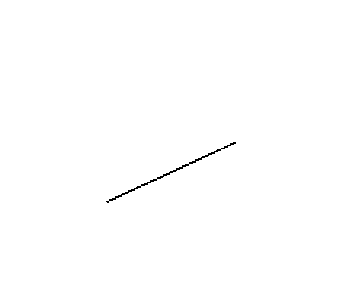
\includegraphics[height=6cm]{Outputs/O1-1.png}
\end{figure}

\textbf{Choose octant: (1 to 8 both inclusive): 1}\\
\textbf{Start point:} (40, 20)
\textbf{End point:} (160, 60)\\
\textbf{Points plotted}: 
(40, 20) (41, 20) (42, 21) (43, 21) 
(44, 21) (45, 22) (46, 22) (47, 22) 
(48, 23) (49, 23) (50, 23) (51, 24) 
(52, 24) (53, 24) (54, 25) (55, 25) 
(56, 25) (57, 26) (58, 26) (59, 26) 
(60, 27) (61, 27) (62, 27) (63, 28) 
(64, 28) (65, 28) (66, 29) (67, 29) 
(68, 29) (69, 30) (70, 30) (71, 30) 
(72, 31) (73, 31) (74, 31) (75, 32) 
(76, 32) (77, 32) (78, 33) (79, 33) 
(80, 33) (81, 34) (82, 34) (83, 34) 
(84, 35) (85, 35) (86, 35) (87, 36) 
(88, 36) (89, 36) (90, 37) (91, 37) 
(92, 37) (93, 38) (94, 38) (95, 38) 
(96, 39) (97, 39) (98, 39) (99, 40) 
(100, 40) (101, 40) (102, 41) (103, 41) 
(104, 41) (105, 42) (106, 42) (107, 42) 
(108, 43) (109, 43) (110, 43) (111, 44) 
(112, 44) (113, 44) (114, 45) (115, 45) 
(116, 45) (117, 46) (118, 46) (119, 46) 
(120, 47) (121, 47) (122, 47) (123, 48) 
(124, 48) (125, 48) (126, 49) (127, 49) 
(128, 49) (129, 50) (130, 50) (131, 50) 
(132, 51) (133, 51) (134, 51) (135, 52) 
(136, 52) (137, 52) (138, 53) (139, 53) 
(140, 53) (141, 54) (142, 54) (143, 54) 
(144, 55) (145, 55) (146, 55) (147, 56) 
(148, 56) (149, 56) (150, 57) (151, 57) 
(152, 57) (153, 58) (154, 58) (155, 58) 
(156, 59) (157, 59) (158, 59) (159, 60) 
(160, 60) 

\newpage
\textbf{Octant 2:}
\begin{figure}[h]
    \centering
    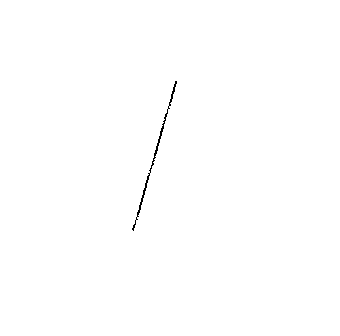
\includegraphics[height=6cm]{Outputs/O2-1.png}
\end{figure}

\textbf{Choose octant: (1 to 8 both inclusive): 2}\\
\textbf{Start point:} (40, 20)
\textbf{End point:} (80, 120)\\
\textbf{Points plotted}: 
(40, 20) (40, 21) (41, 22) (41, 23) 
(42, 24) (42, 25) (42, 26) (43, 27) 
(43, 28) (44, 29) (44, 30) (44, 31) 
(45, 32) (45, 33) (46, 34) (46, 35) 
(46, 36) (47, 37) (47, 38) (48, 39) 
(48, 40) (48, 41) (49, 42) (49, 43) 
(50, 44) (50, 45) (50, 46) (51, 47) 
(51, 48) (52, 49) (52, 50) (52, 51) 
(53, 52) (53, 53) (54, 54) (54, 55) 
(54, 56) (55, 57) (55, 58) (56, 59) 
(56, 60) (56, 61) (57, 62) (57, 63) 
(58, 64) (58, 65) (58, 66) (59, 67) 
(59, 68) (60, 69) (60, 70) (60, 71) 
(61, 72) (61, 73) (62, 74) (62, 75) 
(62, 76) (63, 77) (63, 78) (64, 79) 
(64, 80) (64, 81) (65, 82) (65, 83) 
(66, 84) (66, 85) (66, 86) (67, 87) 
(67, 88) (68, 89) (68, 90) (68, 91) 
(69, 92) (69, 93) (70, 94) (70, 95) 
(70, 96) (71, 97) (71, 98) (72, 99) 
(72, 100) (72, 101) (73, 102) (73, 103) 
(74, 104) (74, 105) (74, 106) (75, 107) 
(75, 108) (76, 109) (76, 110) (76, 111) 
(77, 112) (77, 113) (78, 114) (78, 115) 
(78, 116) (79, 117) (79, 118) (80, 119) 
(80, 120)

\newpage
\textbf{Octant 3:}
\begin{figure}[h]
    \centering
    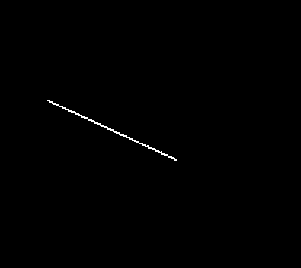
\includegraphics[height=6cm]{Outputs/O3-1.png}
\end{figure}

\textbf{Choose octant: (1 to 8 both inclusive): 3}\\
\textbf{Start point:} (-40, 20)
\textbf{End point:} (-160, 60)\\
\textbf{Points plotted}:
(-40, 20) (-41, 20) (-42, 21) (-43, 21) 
(-44, 21) (-45, 22) (-46, 22) (-47, 22) 
(-48, 23) (-49, 23) (-50, 23) (-51, 24) 
(-52, 24) (-53, 24) (-54, 25) (-55, 25) 
(-56, 25) (-57, 26) (-58, 26) (-59, 26) 
(-60, 27) (-61, 27) (-62, 27) (-63, 28) 
(-64, 28) (-65, 28) (-66, 29) (-67, 29) 
(-68, 29) (-69, 30) (-70, 30) (-71, 30) 
(-72, 31) (-73, 31) (-74, 31) (-75, 32) 
(-76, 32) (-77, 32) (-78, 33) (-79, 33) 
(-80, 33) (-81, 34) (-82, 34) (-83, 34) 
(-84, 35) (-85, 35) (-86, 35) (-87, 36) 
(-88, 36) (-89, 36) (-90, 37) (-91, 37) 
(-92, 37) (-93, 38) (-94, 38) (-95, 38) 
(-96, 39) (-97, 39) (-98, 39) (-99, 40) 
(-100, 40) (-101, 40) (-102, 41) (-103, 41) 
(-104, 41) (-105, 42) (-106, 42) (-107, 42) 
(-108, 43) (-109, 43) (-110, 43) (-111, 44) 
(-112, 44) (-113, 44) (-114, 45) (-115, 45) 
(-116, 45) (-117, 46) (-118, 46) (-119, 46) 
(-120, 47) (-121, 47) (-122, 47) (-123, 48) 
(-124, 48) (-125, 48) (-126, 49) (-127, 49) 
(-128, 49) (-129, 50) (-130, 50) (-131, 50) 
(-132, 51) (-133, 51) (-134, 51) (-135, 52) 
(-136, 52) (-137, 52) (-138, 53) (-139, 53) 
(-140, 53) (-141, 54) (-142, 54) (-143, 54) 
(-144, 55) (-145, 55) (-146, 55) (-147, 56) 
(-148, 56) (-149, 56) (-150, 57) (-151, 57) 
(-152, 57) (-153, 58) (-154, 58) (-155, 58) 
(-156, 59) (-157, 59) (-158, 59) (-159, 60) 
(-160, 60) 


\newpage
\textbf{Octant 4:}
\begin{figure}[h]
    \centering
    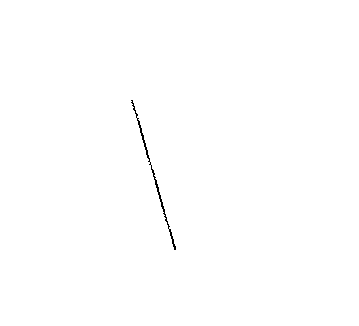
\includegraphics[height=6cm]{Outputs/O4-1.png}
\end{figure}

\textbf{Choose octant: (1 to 8 both inclusive): 4}\\
\textbf{Start point:} (-40, 20)
\textbf{End point:} (-80, 120)\\
\textbf{Points plotted}:
(-40, 20) (-40, 21) (-41, 22) (-41, 23) 
(-42, 24) (-42, 25) (-42, 26) (-43, 27) 
(-43, 28) (-44, 29) (-44, 30) (-44, 31) 
(-45, 32) (-45, 33) (-46, 34) (-46, 35) 
(-46, 36) (-47, 37) (-47, 38) (-48, 39) 
(-48, 40) (-48, 41) (-49, 42) (-49, 43) 
(-50, 44) (-50, 45) (-50, 46) (-51, 47) 
(-51, 48) (-52, 49) (-52, 50) (-52, 51) 
(-53, 52) (-53, 53) (-54, 54) (-54, 55) 
(-54, 56) (-55, 57) (-55, 58) (-56, 59) 
(-56, 60) (-56, 61) (-57, 62) (-57, 63) 
(-58, 64) (-58, 65) (-58, 66) (-59, 67) 
(-59, 68) (-60, 69) (-60, 70) (-60, 71) 
(-61, 72) (-61, 73) (-62, 74) (-62, 75) 
(-62, 76) (-63, 77) (-63, 78) (-64, 79) 
(-64, 80) (-64, 81) (-65, 82) (-65, 83) 
(-66, 84) (-66, 85) (-66, 86) (-67, 87) 
(-67, 88) (-68, 89) (-68, 90) (-68, 91) 
(-69, 92) (-69, 93) (-70, 94) (-70, 95) 
(-70, 96) (-71, 97) (-71, 98) (-72, 99) 
(-72, 100) (-72, 101) (-73, 102) (-73, 103) 
(-74, 104) (-74, 105) (-74, 106) (-75, 107) 
(-75, 108) (-76, 109) (-76, 110) (-76, 111) 
(-77, 112) (-77, 113) (-78, 114) (-78, 115) 
(-78, 116) (-79, 117) (-79, 118) (-80, 119) 
(-80, 120) 


\newpage
\textbf{Octant 5:}
\begin{figure}[h]
    \centering
    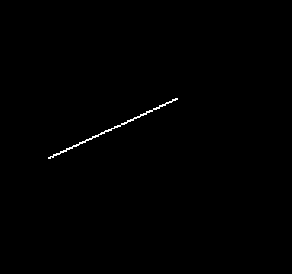
\includegraphics[height=6cm]{Outputs/O5-1.png}
\end{figure}

\textbf{Choose octant: (1 to 8 both inclusive): 5}\\
\textbf{Start point:} (-40, -20)
\textbf{End point:} (-160, -60)\\
\textbf{Points plotted}: 
(-40, -20) (-41, -20) (-42, -21) (-43, -21) 
(-44, -21) (-45, -22) (-46, -22) (-47, -22) 
(-48, -23) (-49, -23) (-50, -23) (-51, -24) 
(-52, -24) (-53, -24) (-54, -25) (-55, -25) 
(-56, -25) (-57, -26) (-58, -26) (-59, -26) 
(-60, -27) (-61, -27) (-62, -27) (-63, -28) 
(-64, -28) (-65, -28) (-66, -29) (-67, -29) 
(-68, -29) (-69, -30) (-70, -30) (-71, -30) 
(-72, -31) (-73, -31) (-74, -31) (-75, -32) 
(-76, -32) (-77, -32) (-78, -33) (-79, -33) 
(-80, -33) (-81, -34) (-82, -34) (-83, -34) 
(-84, -35) (-85, -35) (-86, -35) (-87, -36) 
(-88, -36) (-89, -36) (-90, -37) (-91, -37) 
(-92, -37) (-93, -38) (-94, -38) (-95, -38) 
(-96, -39) (-97, -39) (-98, -39) (-99, -40) 
(-100, -40) (-101, -40) (-102, -41) (-103, -41) 
(-104, -41) (-105, -42) (-106, -42) (-107, -42) 
(-108, -43) (-109, -43) (-110, -43) (-111, -44) 
(-112, -44) (-113, -44) (-114, -45) (-115, -45) 
(-116, -45) (-117, -46) (-118, -46) (-119, -46) 
(-120, -47) (-121, -47) (-122, -47) (-123, -48) 
(-124, -48) (-125, -48) (-126, -49) (-127, -49) 
(-128, -49) (-129, -50) (-130, -50) (-131, -50) 
(-132, -51) (-133, -51) (-134, -51) (-135, -52) 
(-136, -52) (-137, -52) (-138, -53) (-139, -53) 
(-140, -53) (-141, -54) (-142, -54) (-143, -54) 
(-144, -55) (-145, -55) (-146, -55) (-147, -56) 
(-148, -56) (-149, -56) (-150, -57) (-151, -57) 
(-152, -57) (-153, -58) (-154, -58) (-155, -58) 
(-156, -59) (-157, -59) (-158, -59) (-159, -60) 
(-160, -60)

\newpage
\textbf{Octant 6:}
\begin{figure}[h]
    \centering
    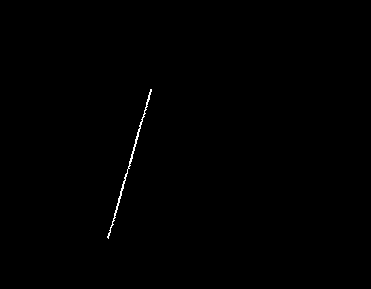
\includegraphics[height=6cm]{Outputs/O6-1.png}
\end{figure}

\textbf{Choose octant: (1 to 8 both inclusive): 6}\\
\textbf{Start point:} (-40, -20)
\textbf{End point:} (-80, -120)\\
\textbf{Points plotted}: 
(-40, -20) (-40, -21) (-41, -22) (-41, -23) 
(-42, -24) (-42, -25) (-42, -26) (-43, -27) 
(-43, -28) (-44, -29) (-44, -30) (-44, -31) 
(-45, -32) (-45, -33) (-46, -34) (-46, -35) 
(-46, -36) (-47, -37) (-47, -38) (-48, -39) 
(-48, -40) (-48, -41) (-49, -42) (-49, -43) 
(-50, -44) (-50, -45) (-50, -46) (-51, -47) 
(-51, -48) (-52, -49) (-52, -50) (-52, -51) 
(-53, -52) (-53, -53) (-54, -54) (-54, -55) 
(-54, -56) (-55, -57) (-55, -58) (-56, -59) 
(-56, -60) (-56, -61) (-57, -62) (-57, -63) 
(-58, -64) (-58, -65) (-58, -66) (-59, -67) 
(-59, -68) (-60, -69) (-60, -70) (-60, -71) 
(-61, -72) (-61, -73) (-62, -74) (-62, -75) 
(-62, -76) (-63, -77) (-63, -78) (-64, -79) 
(-64, -80) (-64, -81) (-65, -82) (-65, -83) 
(-66, -84) (-66, -85) (-66, -86) (-67, -87) 
(-67, -88) (-68, -89) (-68, -90) (-68, -91) 
(-69, -92) (-69, -93) (-70, -94) (-70, -95) 
(-70, -96) (-71, -97) (-71, -98) (-72, -99) 
(-72, -100) (-72, -101) (-73, -102) (-73, -103) 
(-74, -104) (-74, -105) (-74, -106) (-75, -107) 
(-75, -108) (-76, -109) (-76, -110) (-76, -111) 
(-77, -112) (-77, -113) (-78, -114) (-78, -115) 
(-78, -116) (-79, -117) (-79, -118) (-80, -119) 
(-80, -120)


\newpage
\textbf{Octant 7:}
\begin{figure}[h]
    \centering
    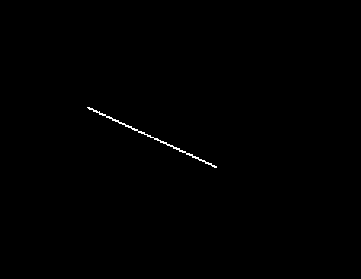
\includegraphics[height=6cm]{Outputs/O7-1.png}
\end{figure}

\textbf{Choose octant: (1 to 8 both inclusive): 7}\\
\textbf{Start point:} (40, -20)
\textbf{End point:} (160, -60)\\
\textbf{Points plotted}:
(40, -20) (41, -20) (42, -21) (43, -21) 
(44, -21) (45, -22) (46, -22) (47, -22) 
(48, -23) (49, -23) (50, -23) (51, -24) 
(52, -24) (53, -24) (54, -25) (55, -25) 
(56, -25) (57, -26) (58, -26) (59, -26) 
(60, -27) (61, -27) (62, -27) (63, -28) 
(64, -28) (65, -28) (66, -29) (67, -29) 
(68, -29) (69, -30) (70, -30) (71, -30) 
(72, -31) (73, -31) (74, -31) (75, -32) 
(76, -32) (77, -32) (78, -33) (79, -33) 
(80, -33) (81, -34) (82, -34) (83, -34) 
(84, -35) (85, -35) (86, -35) (87, -36) 
(88, -36) (89, -36) (90, -37) (91, -37) 
(92, -37) (93, -38) (94, -38) (95, -38) 
(96, -39) (97, -39) (98, -39) (99, -40) 
(100, -40) (101, -40) (102, -41) (103, -41) 
(104, -41) (105, -42) (106, -42) (107, -42) 
(108, -43) (109, -43) (110, -43) (111, -44) 
(112, -44) (113, -44) (114, -45) (115, -45) 
(116, -45) (117, -46) (118, -46) (119, -46) 
(120, -47) (121, -47) (122, -47) (123, -48) 
(124, -48) (125, -48) (126, -49) (127, -49) 
(128, -49) (129, -50) (130, -50) (131, -50) 
(132, -51) (133, -51) (134, -51) (135, -52) 
(136, -52) (137, -52) (138, -53) (139, -53) 
(140, -53) (141, -54) (142, -54) (143, -54) 
(144, -55) (145, -55) (146, -55) (147, -56) 
(148, -56) (149, -56) (150, -57) (151, -57) 
(152, -57) (153, -58) (154, -58) (155, -58) 
(156, -59) (157, -59) (158, -59) (159, -60) 
(160, -60) 

\newpage
\textbf{Octant 8:}
\begin{figure}[h]
    \centering
    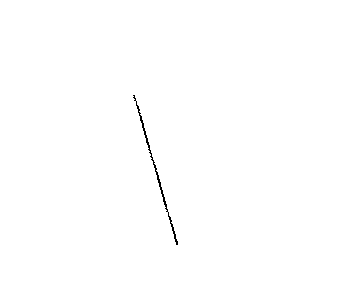
\includegraphics[height=6cm]{Outputs/O8-1.png}
\end{figure}

\textbf{Choose octant: (1 to 8 both inclusive): 8}\\
\textbf{Start point:} (40, -20)
\textbf{End point:} (80, -120)\\
\textbf{Points plotted}: 
(40, -20) (40, -21) (41, -22) (41, -23) 
(42, -24) (42, -25) (42, -26) (43, -27) 
(43, -28) (44, -29) (44, -30) (44, -31) 
(45, -32) (45, -33) (46, -34) (46, -35) 
(46, -36) (47, -37) (47, -38) (48, -39) 
(48, -40) (48, -41) (49, -42) (49, -43) 
(50, -44) (50, -45) (50, -46) (51, -47) 
(51, -48) (52, -49) (52, -50) (52, -51) 
(53, -52) (53, -53) (54, -54) (54, -55) 
(54, -56) (55, -57) (55, -58) (56, -59) 
(56, -60) (56, -61) (57, -62) (57, -63) 
(58, -64) (58, -65) (58, -66) (59, -67) 
(59, -68) (60, -69) (60, -70) (60, -71) 
(61, -72) (61, -73) (62, -74) (62, -75) 
(62, -76) (63, -77) (63, -78) (64, -79) 
(64, -80) (64, -81) (65, -82) (65, -83) 
(66, -84) (66, -85) (66, -86) (67, -87) 
(67, -88) (68, -89) (68, -90) (68, -91) 
(69, -92) (69, -93) (70, -94) (70, -95) 
(70, -96) (71, -97) (71, -98) (72, -99) 
(72, -100) (72, -101) (73, -102) (73, -103) 
(74, -104) (74, -105) (74, -106) (75, -107) 
(75, -108) (76, -109) (76, -110) (76, -111) 
(77, -112) (77, -113) (78, -114) (78, -115) 
(78, -116) (79, -117) (79, -118) (80, -119) 
(80, -120)

\hrule

\end{document}